\documentclass[my_thesis.tex]{subfiles}

\begin{document}
\chapter{3D magnetic equilibria}

The description of a plasma starts with a mathematical model for its equilibrium. In this chapter, we start by discussing the phenomenology of mangetic field equilibrium, and what kind of field line topologies exist in 3D equilibria. We then discuss properties of different equilibrium mathematical models, namely the ideal MHD model, the Taylor state, and the MRxMHD model.

\section{Magnetic field line topologies}
Three dimensional magnetic fields are, in general, composed of  magnetic surfaces, magnetic islands and magnetic field line chaos (see Figure \ref{fig. topology examples}). Measurements in the Wendelstein-7X stellarator via injection of an electron beam in a dilute gas \citep{pedersenConfirmationTopologyWendelstein2016} showed experimentally the existance of magnetic surfaces (Figure \ref{fig w7x magnetic surface}) and of the edge magnetic island chain (Figure \ref{fig w7x magnetic island}).

\begin{figure}%
	\centering
	\subfloat[Magnetic surface]{\label{fig w7x magnetic surface}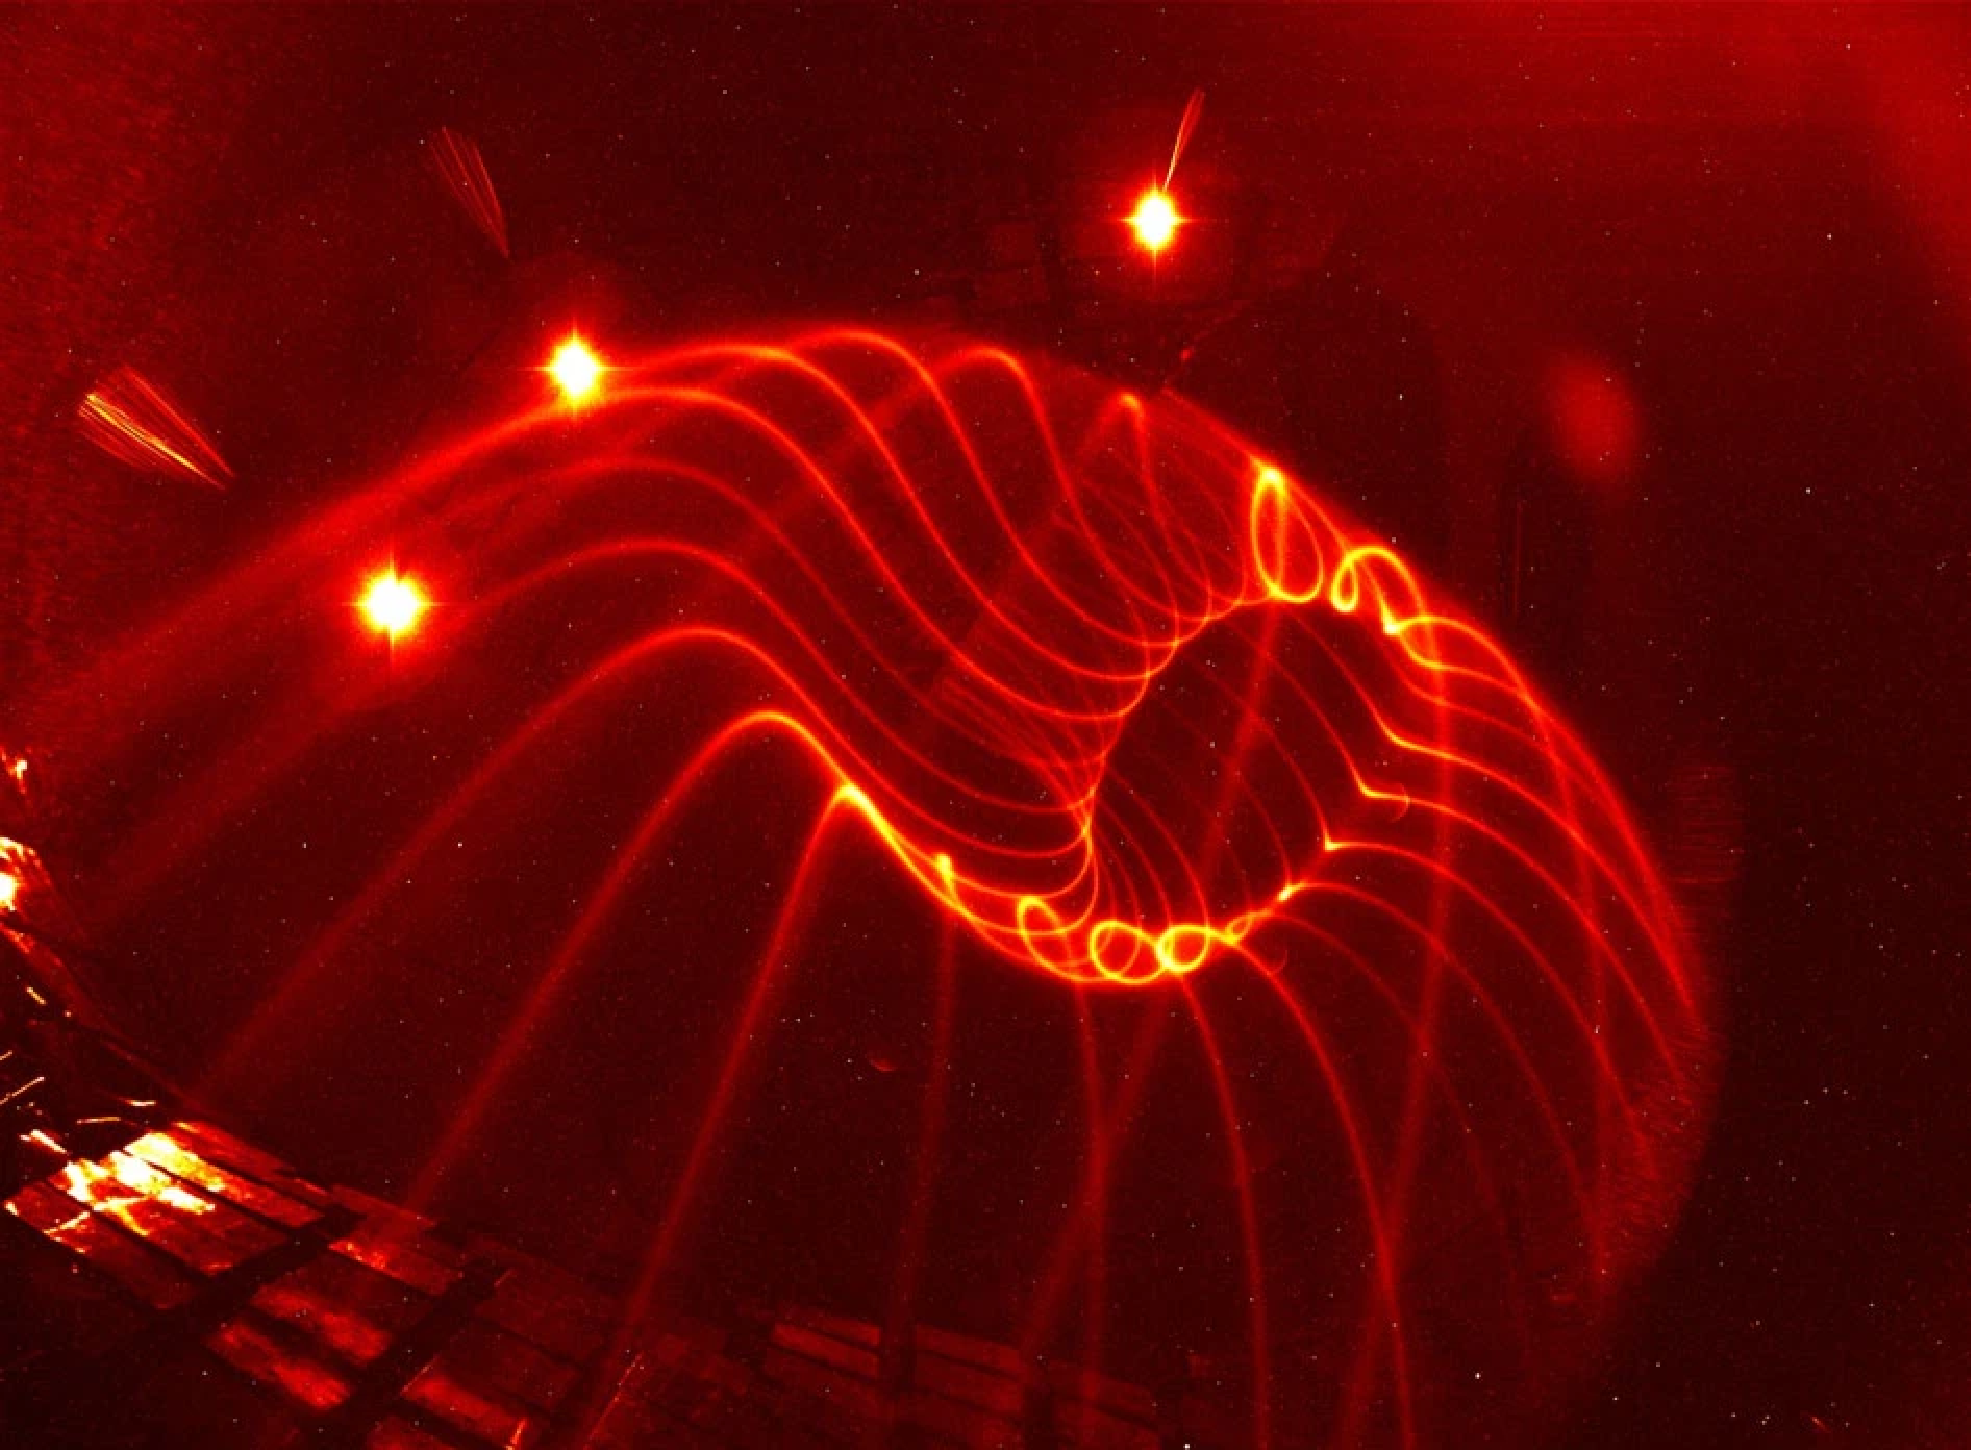
\includegraphics[height=4.8cm]{images/Pedersen2016_MagneticSurface_W7X.pdf}}%
	\qquad
	\subfloat[Magnetic islands]{\label{fig w7x magnetic island}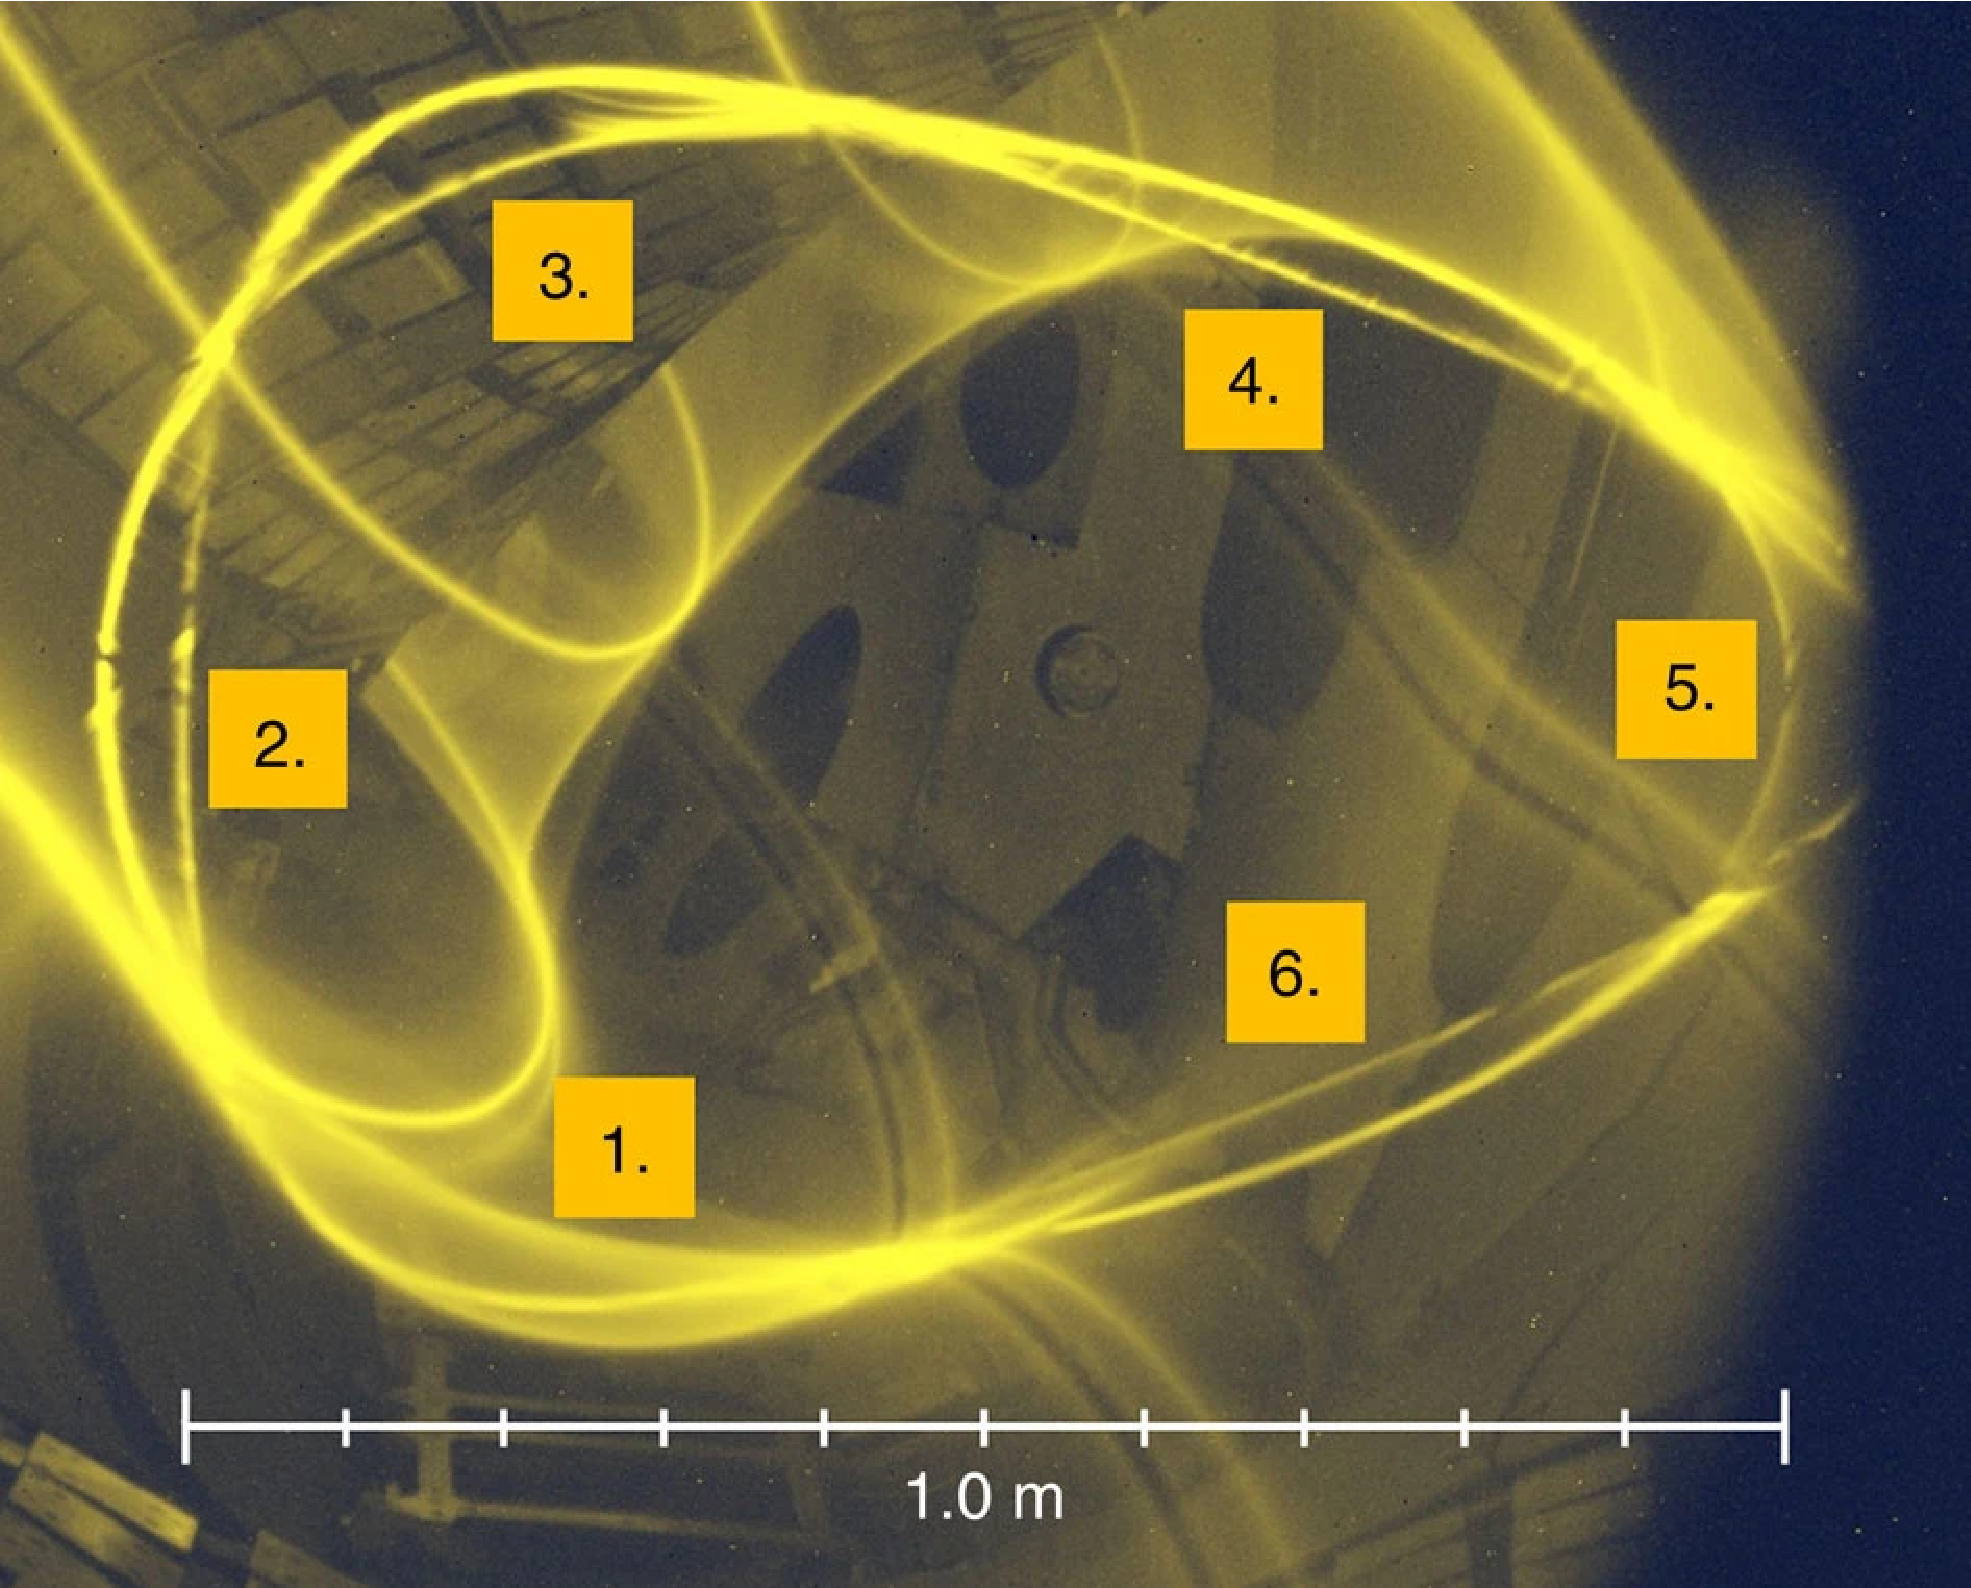
\includegraphics[height=4.8cm]{images/Pedersen2016_MagneticIsland_W7X.pdf}}
	\caption{Measurement of the field line topology in W7-X via injection of an electron beam in a dilute gas \citep{pedersenConfirmationTopologyWendelstein2016}.}
	\label{fig. w7x topology measurement}%
\end{figure}

Now, suppose that an equilibrium is given --- by that, we mean that the magnetic field $\mathbf{B}$ is known everywhere, \textit{i.e.} at any position $(r,\theta,\phi)$, where r is a radial coordinate, $\theta$ is a poloidal angle and $\phi$ is the usual cylindrical toroidal angle. To visually see the magnetic field line topologies, a Poincare section can be plotted. To do so, the field line is followed by solving the differential equation
\begin{equation}
	\frac{d\theta}{d\phi} = \frac{\mathbf{B}\cdot\nabla\theta}{\mathbf{B}\cdot\nabla\phi},
\end{equation}
with initial condition $r(0)=r_0$, $\theta(0)=\theta_0$ where $(r_0,\theta_0)$ are the initial field line position at $\phi=0$. An example of a field line followed on a magnetic surface is shown on Figure \ref{fig. field line tracing}. The field line is followed for multiple toroidal transits, and its position $(r_k,\theta_k)$ is saved whenever $\phi=2k\pi$, with $k\in\mathbb{N}$. The Poincare section is then plotted on the $(R,Z)$ plane. An example of a Poincare section with different field line topologies is shown on Figure \ref{fig topology examples}.

\begin{figure}
	\centering
	\subfloat[][Field line]{\label{fig. field line tracing}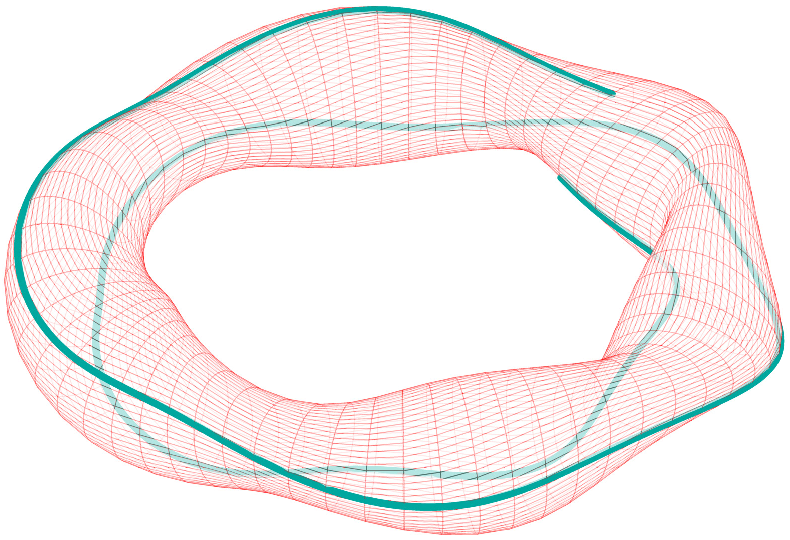
\includegraphics[height=4cm]{images/3d_field_line_tracing.pdf}}
	\hfill
	\subfloat[][Poincare section]{\label{fig. topology examples}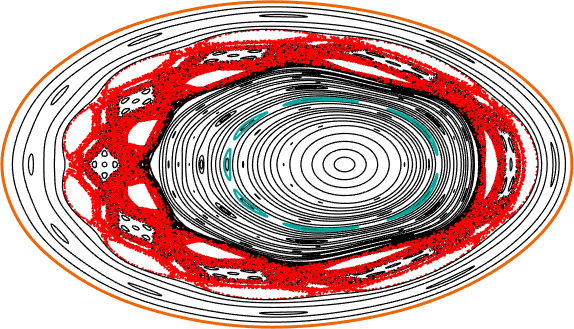
\includegraphics[height=4cm]{images/poincare_section_example.pdf}}
	\caption{Example of field line tracing and Poincare section in a rotating ellipse. Left: 3D mesh of a magnetic surface (red) and a traced field line over two periods (blue). Right: Poincare section of multiple field lines, a magnetic surface (orange), a magnetic island (blue) and a chaotic field line (red).}
	\label{fig poincare section}
\end{figure}

%Magnetic surfaces are toroidal surfaces on which the magnetic lays, \textit{i.e.} $\mathbf{B}\cdot\mathbf{n}=0$ with $\mathbf{n}$ a vector normal to the magnetic surface. In axisymmetric devices such as tokamaks, one can prove that nested magnetic surfaces exist everywhere, from the plasma edge to the magnetic axis, which is the innermost field line. Magnetic islands are formed when (i) the magnetic field is perturbed with a mode $\delta B_r \propto exp(i(m\theta-n\phi))$, with $(\theta,\phi)$ a poloidal and toroidal angle, and $m$, $n$ the poloidal and toroidal mode number, and (ii) the rotational transform is a rational number equal to $\iotabar=n/m$. Finally, magnetic field line chaos is formed when two or more island chains overlap --- this is the so-called Chirikov criterion \citep{Chirikov1979}. Further details about these magnetic field line topologies and their hamiltonian description can be found in the review paper by \citet{Meiss1992c} and references therein. 

To accurately model and understand the physics in a stellarator, it is important to consider equilibria that allow magnetic islands and magnetic field line topologies. In what follows, we discuss important properties of the ideal \ac{MHD} model (section \ref{section ideal mhd}), the Taylor relaxation model (section \ref{section taylor state}) and of the \ac{MRxMHD} model (section \ref{section mrxmhd}).

%At zeroth order, particle and energy confinement is obtained on magnetic surfaces; magnetic islands and magnetic field line chaos, on the other hand, may increase radial transport. This is not the full story; structures in regions occupied by chaotic field lines can potentially support pressure gradient \citep{Hudson2008}, but in general the transport in these regions will be greater than in regions occupied by magnetic surfaces. 

% \begin{figure}
% \centering
% 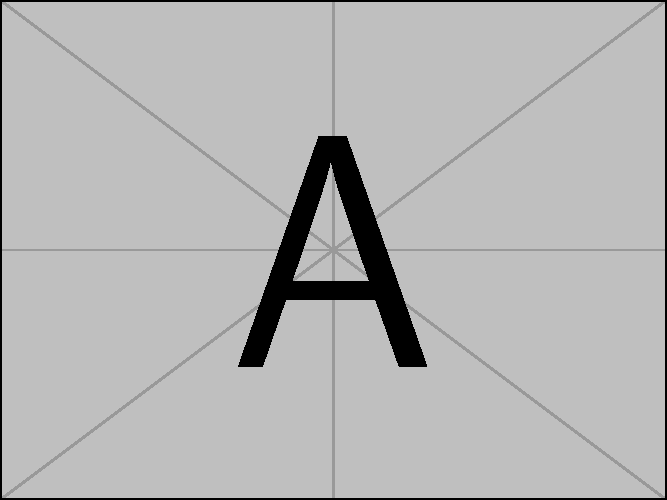
\includegraphics[width=\linewidth]{images/example-image-a.pdf}
% \caption{Example of a magnetic surface, a magnetic island chain and magnetic field line chaos.}
% \label{fig. topology examples}
% \end{figure}

%In the next sections, we will discuss different mathematical models that have been developed to describe 3D magnetic equilibria, \textit{i.e.} answering the question "\emph{Given a boundary, pressure and current profiles, what is the magnetic field in a plasma?}"




\section{Ideal MHD}
\label{section ideal mhd}
Ideal \ac{MHD} is probably the most well-known and used model to describe macroscopic plasma equilibria. It aims at describing slow phenomena on macroscopic scales. Quasi-neutrality is assumed, \textit{i.e.} $n_e=n_i=n$, where $n_e$ and $n_i$ are the electron and ion densities respectively. The plasma is modeled with a single fluid approximation, where the pressure is isotropic and defined as the sum of the ion and electron pressure, $p=p_i+p_e=2nT$, and the temperature is defined as the average of the ion and electron temperature, $T=(T_i+T_e)/2$. In addition, it is assumed that electromagnetic waves have phase velocities negligible in comparison to the speed of light, $\omega/k\ll c$, the thermal velocities of ions and electrons are non-relativistic, $v_{Ti}\ll v_{Te}\ll c$, with $v_{Ti}=(kT_i/m_i)^{1/2}$, $k$ is Boltzmann constant, and $m_i$ the ion mass. Phenomena described by ideal MHD have frequencies smaller than the electron plasma frequency, $\omega\ll \omega_{pe}=(n_ee^2/m_e\epsilon_0)^{1/2}$, where $e$ the elementary charge, $m_e$ the electron mass and $\epsilon_0$ the vacuum permittivity, and have characteristic length larger than the Debye length, $a\gg \lambda_D=(kT_e/4\pi n_e e^2)^{1/2}$. Finally, electron inertia is neglected, \textit{i.e.} their response to a force is instantaneous.

The ideal \ac{MHD} equations are \citep{Freidberg2014},
\begin{align}
	\frac{\partial \rho}{\partial t} + \nabla\cdot(\rho\mathbf{v}) &= 0 \label{mass equation}\\
	\rho\frac{d\mathbf{v}}{dt} &= \mathbf{J}\times\mathbf{B} - \nabla p \label{momentum equation}\\
	\frac{d}{dt}\left(\frac{p}{\rho^\gamma}\right) &= 0 \label{energy equation}\\
	\mathbf{E} + \mathbf{v}\times\mathbf{B} &= 0 \label{ideal Ohms law}\\
	\nabla\times\mathbf{B} &=\mu_0\mathbf{J} \label{equation ampere}\\
	\nabla\cdot\mathbf{B}&=0 \label{equation div B}\\
	\nabla\times\mathbf{E}&=-\frac{\partial \mathbf{B}}{\partial t}, \label{equation rot E}
\end{align}
where $\mathbf{J}$ and $\rho$ are the current and mass densities, $\mu_0=4\pi 10^{-7}$ is the vacuum permeability, $\mathbf{E}$ is the electric field and $\mathbf{v}$ is the fluid velocity. Note that Ampere's law, Eq.(\ref{equation ampere}), implies charge conservation,
\begin{equation}
	\nabla\cdot\mathbf{J} = 0\label{equation charge conservation}
\end{equation}

At equilibrium, all time derivatives vanish ($\partial/\partial t = 0$), and assuming zero flow ($\mathbf{v}=0$), we get the \emph{ideal MHD equilibrium equations},
\begin{align}
	\mathbf{J}\times\mathbf{B} &= \nabla p \label{equation perp force balance}\\
	\nabla\times\mathbf{B} &=\mu_0\mathbf{J}\\
	\nabla\cdot\mathbf{B}&=0.\label{equation div B ideal mhd}
\end{align}
Analytical solutions to the equations (\ref{equation perp force balance})-(\ref{equation div B ideal mhd}) can be found in different geometries; an example is cylindrical geometry is provided in appendix \ref{appendix jxb=grad p solution}.

Equation (\ref{equation perp force balance}) implies that $\mathbf{B}\cdot\nabla p=0$, \textit{i.e.} the pressure is constant along a field line. If the pressure profile is smooth and not constant in any region, then equation ()\ref{equation perp force balance}) implies that magnetic field lays on surfaces of constant pressure, \textit{i.e.} the magnetic surfaces. The existence of magnetic  surfaces where $\nabla p\neq 0$ is however the source of diverging currents, as we shall discuss in the next sections.



% ================================================ CURRENTS ================================================
\subsection{Currents in ideal MHD equilibria}
The current density can be written as the sum of a component parallel to the magnetic field $J_\parallel \hat{\mathbf{b}}$, with $\hat{\mathbf{b}}=\mathbf{B}/B$ and of a component perpendicular to the magnetic field $\mathbf{J}_\perp$.

Following \citet{Helander2014}, the perpendicular component is required to counter-balance the pressure gradient in the force balance, \textit{i.e.} taking the cross product of $\mathbf{B}$ with Eq.(\ref{equation perp force balance}), we get
\begin{equation}
	\mathbf{J}_\perp = \frac{\mathbf{B}\times\nabla p}{\mathbf{B}^2}.
\end{equation}
Parallel current $J_\parallel$ are then generated to ensure charge conservation (Eq.(\ref{equation charge conservation})). Imposing $\nabla \cdot (J_\parallel\mathbf{\hat{b}}) = - \nabla\cdot\mathbf{J}_\perp$ leads to 
\begin{equation}
	J_\parallel = u(\psi_t,\theta,\phi)\frac{dp}{d\psi_t}B + \frac{\langle J_\parallel B\rangle B}{\langle B^2\rangle},
\end{equation}
where $(\psi_t,\theta,\phi)$ are the toroidal flux, a poloidal angle and a toroidal angle, and $\langle\cdot\rangle$ denotes a flux surface average. The function $u(\psi_t,\theta,\phi)$ satisfies
\begin{equation}
	\mathbf{B}\cdot\nabla u = -(\mathbf{B}\times\nabla\psi_t)\cdot\nabla\left(\frac{1}{B^2}\right). \label{eq.diff_u}
\end{equation}
The total current density is thus
\begin{equation}
	\mathbf{J} = \frac{\mathbf{B}\times\nabla p}{\mathbf{B}^2} + \left(u(\psi_t,\theta,\phi)\frac{dp}{d\psi_t} + \frac{\langle J_\parallel B\rangle}{\langle B^2\rangle}\right)\mathbf{B}, \label{equation current density}
\end{equation}
where the first term on the right hand side of Eq.(\ref{equation current density}) is the \emph{diamagnetic current}, the second is the \emph{Pfirsch-Schl\"uter current} and the last term encompasses other parallel currents, such as the externally driven currents (Ohmic, \ac{ECCD}, \ac{NBCD}) or bootstrap current.




% ================================================ CLASSES OF EQUILIBRIA ================================================
\subsection{Classes of well posed 3D magnetic equilibria}

As we shall see, the magnetic differential equation \ref{eq.diff_u} has important implications on the existence of 3D magnetic equilibria with nested magnetic surfaces. In the discussion below, we follow \citet{Helander2014} and solve equation (\ref{eq.diff_u}) assuming the existence of magnetic surfaces and using the coordinate system $(\psi_t,\theta_b,\phi_b)$, where $(\theta_b,\phi_b)$ are the poloidal and toroidal Boozer angles (see appendix \ref{appendix boozer coordinates}). We write the functions $u(\psi_t,\theta_b,\phi_b)$ and $B^{-2}(\psi_t,\theta_b,\phi_b)$ as Fourier series,
\begin{align}
	u(\psi_t,\theta_b,\phi_b) &= \sum_{m,n} u_{mn}(\psi_t) e^{i(m\theta_b-n\phi_b)}\\
	\frac{1}{B^2}(\psi_t,\theta_b,\phi_b) &= \sum_{m,n} h_{mn}(\psi_t) e^{i(m\theta_b-n\phi_b)}.
\end{align}
Writing $\mathbf{B}$ as
\begin{equation}
	\mathbf{B} = I(\psi_t)\nabla\theta_b + G(\psi_t)\nabla\phi_b + K(\psi_t,\theta_b,\phi_b)\nabla\psi_t,
\end{equation}
we obtain for the right hand side of Eq.(\ref{eq.diff_u})
\begin{align}
	\mathbf{B}\cdot\nabla u &= \mathbf{B}\cdot\nabla\theta_b\frac{\partial u}{\partial \theta_b} + \mathbf{B}\cdot\nabla\phi_b\frac{\partial u}{\partial \phi_b} + \mathbf{B}\cdot\nabla\psi_t\frac{\partial u}{\partial \psi_t} \\
	&= \left(\iotabar \frac{\partial u}{\partial \theta_b} + \frac{\partial u}{\partial \phi_b}\right)\mathbf{B}\cdot\nabla\phi_b,
\end{align}
and for the left hand side
\begin{align}
	\left(\mathbf{B}\times\nabla\psi_t\right)\cdot\nabla \frac{1}{B^2} &= \left(I\nabla\theta_b\times\nabla\psi_t + G\nabla\phi_b\times\nabla\psi_t\right)\cdot\nabla\frac{1}{B^2}\\
	&= \frac{1}{\sqrt{g}}\left(G\frac{\partial}{\partial\theta_b} - I \frac{\partial}{\partial \phi_b}\right)\frac{1}{B^2},
\end{align}
with $(\nabla\psi_t\cdot(\nabla\theta_b\times\nabla\phi_b))^{-1} = \sqrt{g}$ the Boozer coordinate jacobian. Substituting the Fourier series for $u$ and $1/B^2$, we finally obtain
\begin{equation}
	(m\iotabar - n)u_{mn} = \frac{1}{\sqrt{g}}\frac{1}{\mathbf{B}\cdot\nabla\phi_b}(mG + nI)h_{mn}.
\end{equation}
Rearranging the terms, we get an expression for $u_{mn}$,
\begin{equation}
	u_{mn} = \frac{1}{\sqrt{g}}\frac{1}{\mathbf{B}\cdot\nabla\phi_b}\frac{(mG + nI)}{m\iotabar - n}h_{mn} + \Delta_{mn}\delta(\psi_t-\psi_{t,mn}),
\end{equation}
where $\Delta_{mn}$ is an arbitrary constant and $\psi_{t,mn}$ is the toroidal flux enclosed by a magnetic surface where $\iotabar=n/m$. The Pfirsch-Schl\"uter current density (Eq.(\ref{equation current density})) has then two parts; one is a delta function, and the other is
\begin{equation}
	J_{mn} = \frac{1}{\sqrt{g}}\frac{1}{\mathbf{B}\cdot\nabla\phi_b}\frac{(mG + nI)}{m\iotabar - n}h_{mn}p'(\psi_t).\label{diverging current}
\end{equation}

We see that at rational surfaces ($\iotabar=n/m$), the current density (\ref{diverging current}) diverges as a $1/x$ singularity if the pressure gradient is finite. This is not physical since the integrated net toroidal current would diverge as well. To circumvent this issue and obtain well defined, ideal MHD solutions, one has to consider constrained classes of equilibria.
\begin{enumerate}
	\item One possibility is to consider equilibria where the inverse magnetic field squared resonant harmonic is zero at each rational surface, \emph{i.e.} $h_{mn}=0$, discussed by \citet{Weitzner2014}.
	\item Another is to relax the assumption of smooth, continuous solutions, and consider rotational transform profiles that are stepped --- essentially jumping from irrational to irrational values, and entirely avoiding rational surfaces. This has been discussed by \citet{Loizu2015a}.
	\item Similarly, one could consider equilibria where the pressure is constant around resonant surfaces. Since rationals are dense in $\mathbb{R}$, the pressure profile is either stepped or fractal. Stepped pressure equilibria have been proven to exist close to axisymmetry by \citet{Bruno1996}.
	\item Finally, a combination of the second and third class discussed above, where the rotational transform profile and the pressure profile are alternatively constant, can be constructed to obtain solution with continuous but non-smooth solutions \citep{Hudson2017a}
\end{enumerate}
In what follows, we will work with the third class of equilibria described above, namely stepped-pressure equilibria. The reason is three-fold: (i) these equilibria are numerically tractable, (ii) solutions with magnetic islands and chaos can be obtained and (iii) solutions have been proven to exist under some conditions. In particular, we will look at \ac{MRxMHD} equilibria, which can be seen as a combination of Taylor states, described in section \ref{section taylor state}.



\section{Taylor state}
\label{section taylor state}
One trivial way to solve the ideal MHD equation (\ref{equation perp force balance})-(\ref{equation div B ideal mhd}) is to consider the case where the pressure is flat, \textit{i.e.} $p'=0$. There are thus no "1/x" singular current densities as in equation (\ref{diverging current}). The force balance equation (\ref{equation perp force balance}) implies that $\mathbf{J}\times\mathbf{B}=0$, meaning that the current density is parallel to the magnetic field, $\mathbf{J}=\mu(r,\theta,\phi)\mathbf{B}$.

The Taylor state \citep{Taylor1974,Taylor1986} is a particular case of force-free fields where the function $\mu$ is a constant, which give the Taylor equilibrium equation
\begin{equation}
	\nabla\times\mathbf{B}=\mu\mathbf{B}. \label{equation Taylor state}
\end{equation}

Solution to the equation (\ref{equation Taylor state}) in a slab and a cylinder are provided in appendix \ref{appendix taylor state}.


\section{MRxMHD}
\label{section mrxmhd}
%The \ac{MRxMHD} theory \citep{Dewar2015, Hole2006} has been developed to address this question. \ac{MRxMHD} minimizes the \ac{MHD} energy functional \citep{kruskal_equilibrium_1958} while keeping the magnetic helicity and the magnetic fluxes constant \citep{Dewar2015} in a finite set of $N_{vol}$ nested volumes $\mathcal{V}_l$ at constant pressure (see Figure \ref{fig:Illustration_SPEC}) but otherwise allowing arbitrary, non-ideal variations in the magnetic field. Interfaces $\delta\mathcal{V}_l$ separating the volumes are ideal flux surfaces which therefore cannot undergo magnetic re-connection, effectively constraining discretely the magnetic field topology. In the limit of a single volume, $N_{vol}=1$, Taylor states \citep{Taylor1974, Taylor1986} are recovered, while in the limit of an infinite number of volumes, $N_{vol}\rightarrow\infty$, it has been proven that \ac{MRxMHD} recovers ideal \ac{MHD} (section \ref{section ideal mhd}) \citep{Dennis2013} in the limit of continuously nested flux surfaces, thereby bridging the gap between both theories.

Taylor states can not describe plasma equilibria with pressure profile. An alternative is proposed by the MRxMHD equilibrium model, which describes solutions to equations (\ref{equation perp force balance})-(\ref{equation div B ideal mhd}) assuming stepped-pressure profiles. The pressure steps are supported by magnetic surfaces $\mathcal{I}_l$, $l\in\{1,\ldots,N_{vol}\}$, with irrational rotational transform, \textit{i.e.} $\iotabar\in\mathbb{R}\setminus\mathbb{Z}$, which defines a finite number of volumes $\mathbf{V}_l$ between each couple of interface (see Figure \ref{fig:Illustration_SPEC}). In each volume, the magnetic field is described by a Taylor state, 
\begin{equation}
	\nabla\times\mathbf{B}=\mu_l\mathbf{B}. \label{eq.BeltramiEquation}
\end{equation}
In addition, the total pressure (plasma and magnetic pressure) is required to be continuous across each volume interface $\mathcal{I}_l$,
\begin{equation}
	\left[\left[p + \frac{B^2}{2\mu_0}\right]\right]_l = 0, \label{eq.force_balance}
\end{equation}
where $[[x]]_l\equiv x_{l+1}-x_l$ denotes the discontinuity across interface $l^{\text{th}}$. The MRxMHD equilibrium can then be seen as a collection of nested Taylor state at equilibrium with one another. 

\begin{figure}
	\centering
	\begin{tikzpicture}
		\node[] (fig) at (0,0)
		{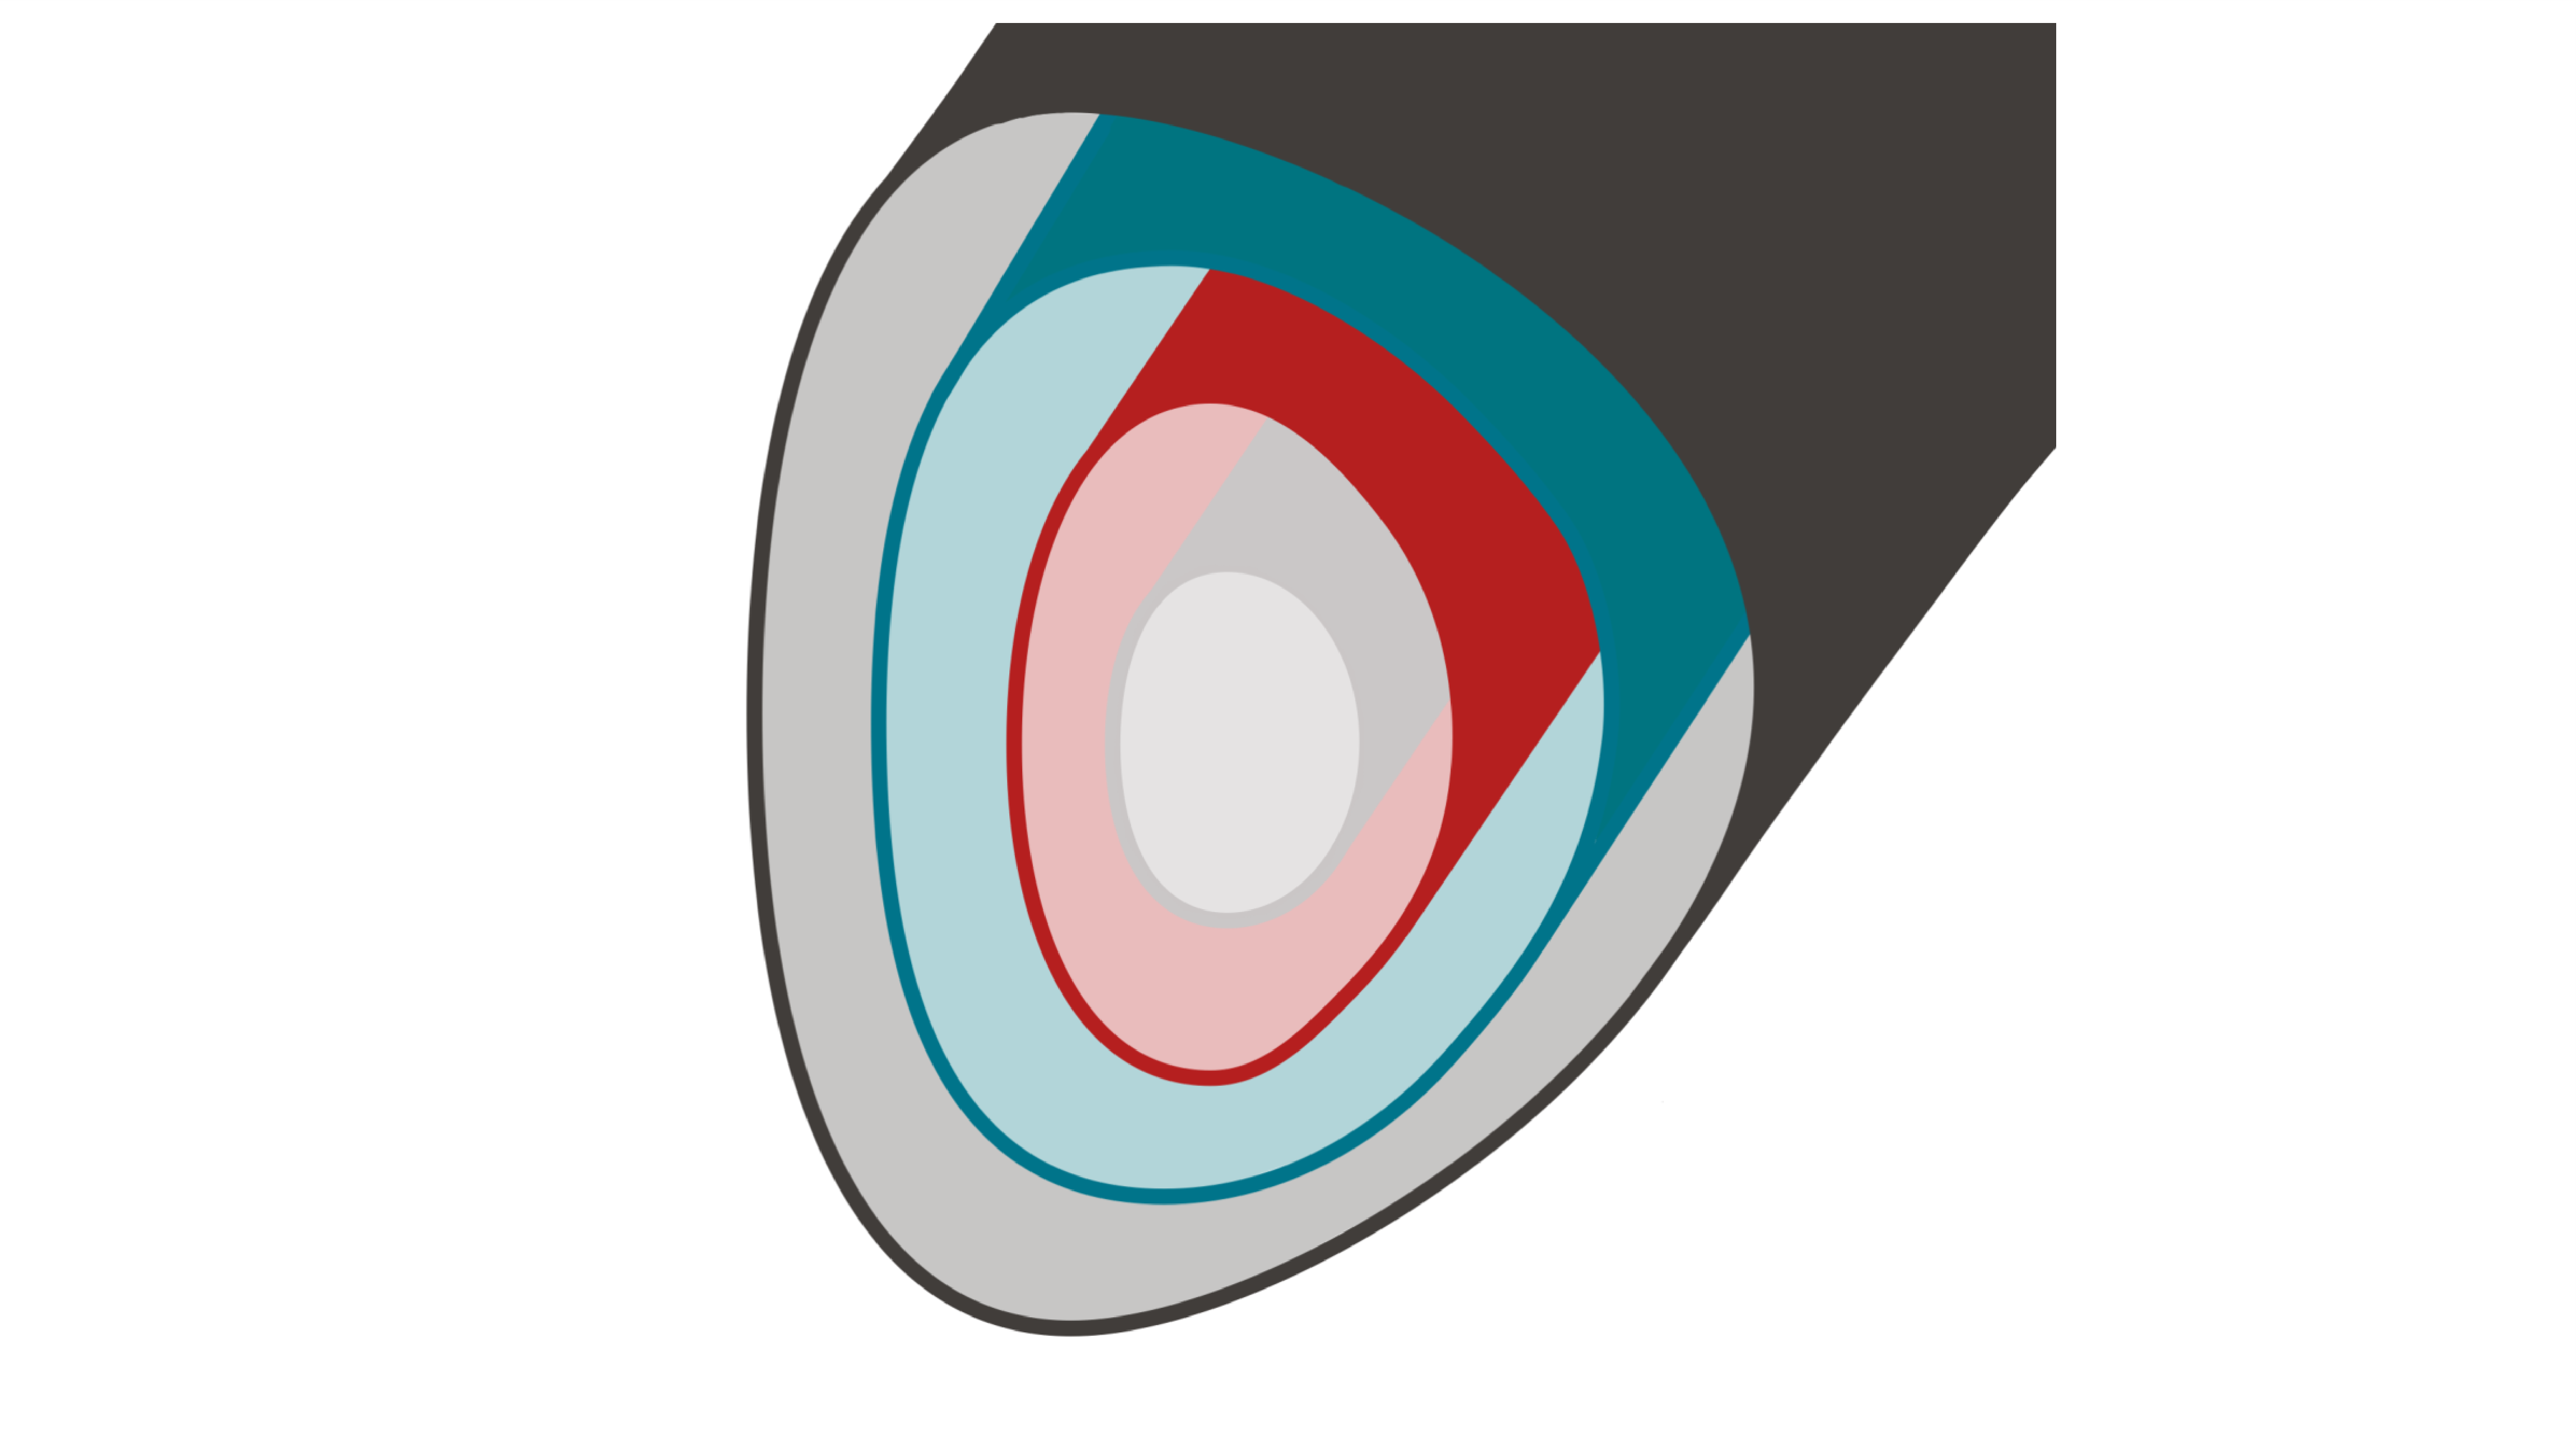
\includegraphics[width=0.9\textwidth]{main/Figures_CurrentConstraint/ABaillod_fig1.pdf}};
		%\draw (-5,-5) grid[] (5,5);
		\draw (-0.3 ,-0.3 ) node {$\mathcal{V}_1$};
		\draw (-0.9 ,-0.9 ) node {$\mathcal{V}_2$};
		\draw (-1.35 ,-1.35) node {$\mathcal{V}_3$};
		\draw (-1.9 ,-1.9 ) node {$\mathcal{V}_4$};
		\draw ( 0.0 , 1.0 ) node {$\mathcal{I}_1$};
		\draw ( 0.5 , 1.5 ) node {\color{white}$\mathcal{I}_2$};
		\draw ( 0.85 , 1.85 ) node {\color{white}$\mathcal{I}_3$};
		\draw ( 1.5 , 2.5 ) node {\color{white}$\mathcal{I}_4$};
	\end{tikzpicture}
	\caption{Illustration of 4 nested volumes, $\mathcal{V}_1$ to $\mathcal{V}_4$, separated by 4 interfaces, $\mathcal{I}_1$ to $\mathcal{I}_4$.}
	\label{fig:Illustration_SPEC}
\end{figure}

In each volume $\mathcal{V}_l$, the solution to Eq.(\ref{eq.BeltramiEquation}) is completely determined by three scalars (for example $\{\mu_l,\psi_{t,l},\psi_{p,l}\}$), the geometry of interfaces bounding the volume and a boundary condition for the magnetic field normal to the interfaces $\mathbf{B}_l\cdot\hat{\mathbf{n}}_k$, $k=\{l-1,l\}$, with $\hat{\mathbf{n}}_k$ a unit vector perpendicular to the interface $k$. In \ac{MRxMHD}, the interfaces are imposed to be flux surfaces, with $\mathbf{B}_l\cdot\hat{\mathbf{n}}_k=0$. In the innermost volume, which is topologically different from the others, only two scalars are required in addition to the geometrical degrees of freedom and the condition $\mathbf{B}_1\cdot\hat{\mathbf{n}}_1=0$.



\subsection{Currents in MRxMHD}
One important part of the work presented in this thesis is the implementation of a new capability in the SPEC code (introduced in the next chapter) to run at fixed net toroidal current profile. The numerical implementation will be explained in great details in section \ref{sec. current constraint}; we describe in this section how currents are represented in the MRxMHD theory. This section has been part of a publication by \citet{Baillod2021}.

In \ac{MRxMHD}, two spatially distinct net toroidal current profiles co-exist, namely currents flowing in the volumes, $\{I^v_{l,\phi}\}_{l=\{1,\ldots,N_{vol}\}}$, and surface currents flowing at the volumes' interfaces, $\{I^s_{l,\phi}\}_{l=\{1,\ldots,N_{vol}-1\}}$ (current sheets), where the subscript $\phi$ refers to the toroidal angle. The volume current $I^v_{l,\phi}$ in volume $\mathcal{V}_l$ is easily evaluated using Eq.(\ref{eq.BeltramiEquation}) and Ampere's law,
\begin{equation}
    \mu_0I^v_{l,\phi} = \mu_l\iint_{\mathcal{S}_{l,\phi}} \mathbf{B}\cdot\mathbf{dS}_{l,\phi} = \mu_l \psi_{t,l},
    \label{eq.volume_current}
\end{equation}
where $\mathcal{S}_{l,\phi}$ is a constant-$\phi$ surface in volume $\mathcal{V}_l$ and $\mathbf{dS}_{l,\phi}$ is the differential surface element normal to $\mathcal{S}_{l,\phi}$. Volume currents include externally driven currents such as \ac{ECCD}, \ac{NBCD} or Ohmic current. Eq.(\ref{eq.volume_current}) might be surprising since toroidal currents are usually expressed in terms of functions of the poloidal fluxes and not the toroidal fluxes. In essence, the poloidal flux dependence is contained in $\mu_l$, which is related to the parallel current density, as $\mu_l = \mu_0 \mathbf{j}_l\cdot\mathbf{B}_l / B_l^2$, with $\mathbf{j}_l$ the current density in volume $\mathcal{V}_l$. The surface current $I^s_{l,\phi}$ at interface $\mathcal{I}_l$ can be evaluated using Ampere's law
\begin{equation}
    \mu_0I^s_{l,\phi} = \int_{\Gamma _l} \left[\left[ \mathbf{B} \right]\right]_l \cdot \mathbf{dl} = \oint_0^{2\pi} \left[\left[B_\theta\right]\right] d\theta \equiv 2\pi \left[\left[ \tilde{B}_{\theta} \right]\right]_l, \label{eq.surf_current}
\end{equation}
where $\Gamma_l$ is a closed curve following the interface $\mathcal{I}_l$ poloidally and $\tilde{B}_{\theta}$ is the $m=n=0$ Fourier mode of the covariant component of the poloidal magnetic field. In Eq.(\ref{eq.surf_current}), the poloidal and toroidal angles, $\theta$ and $\phi$, are as-of-yet arbitrary. However the surface currents $I^s_{l,\phi}$ are, as expected, independent of these angles choice, since the surface currents only depend on the $m=n=0$ mode of the field. Surface currents represent all equilibrium pressure-driven currents, such as diamagnetic, Pfirsch-Schl\"uter, and bootstrap currents, as well as shielding currents arising when an ideal interface is positioned on a resonance \citep{Loizu2015}.

As a side note, we remark that while ideal \ac{MHD} equilibria are defined by two free functions (\textit{e.g.} the pressure and the rotational transform profiles, $p(\psi_t)$ and $\iotabar(\psi_t)$, or the pressure and the current profiles, $p(\psi_t)$ and $I_\phi(\psi_t)$), \ac{MRxMHD} requires two scalars to determine the solution in a volume $\mathcal{V}_l$, in addition to the pressure and toroidal flux. This can be considered as three independent discrete profiles that are required to determine an equilibrium. Examples are $\{p_l, \mu_l, \psi_{p,l}\}_{l=1,\ldots,N_{vol}}$, $\{p_l, \mu_l, K_l\}_{l=1,\ldots,N_{vol}}$ or $\{p_l,\iotabar^-_l,\iotabar^+_l\}_{l=1,\ldots,N_{vol}}$, with $\iotabar^\pm_l$ the rotational transform on the inner and outer side of the interface $\mathcal{I}_l$, or $\{p_l,I^v_{l,\phi},I^s_{l,\phi}\}_{l=1,\ldots,N_{vol}}$, as functions of $\{\psi_{t,l}\}_{l=1,\ldots,N_{vol}}$.


\subsection{Currents discretization}
Typically, continuous current profiles are provided by analytical models or after equilibrium reconstruction using experimental data. We now discuss how these profiles can be represented in the framework of \ac{MRxMHD}. Consider an externally driven current profile, \textit{e.g} \ac{ECCD}, provided as the enclosed toroidal current as a function of the toroidal magnetic flux, \textit{i.e.} $I_{\phi,ECCD}(\psi_t)$, and a pressure-driven current profile, \textit{e.g.} the bootstrap current, provided similarly as the enclosed toroidal current as a function of the toroidal flux, $I_{\phi,BS}(\psi_t)$. We also assume that the pressure profile, $p(\psi_t)$, the number of volumes, $N_{vol}$, and their enclosed toroidal fluxes, $\{\psi_{t,l}\}_{l=1,\ldots,N_{vol}}$, are given (see Figure \ref{fig:sketch_pressure}). The question of how many volumes and where to position their interfaces to best represent a given pressure profile is not addressed in this paper.

\begin{figure}
    \centering
    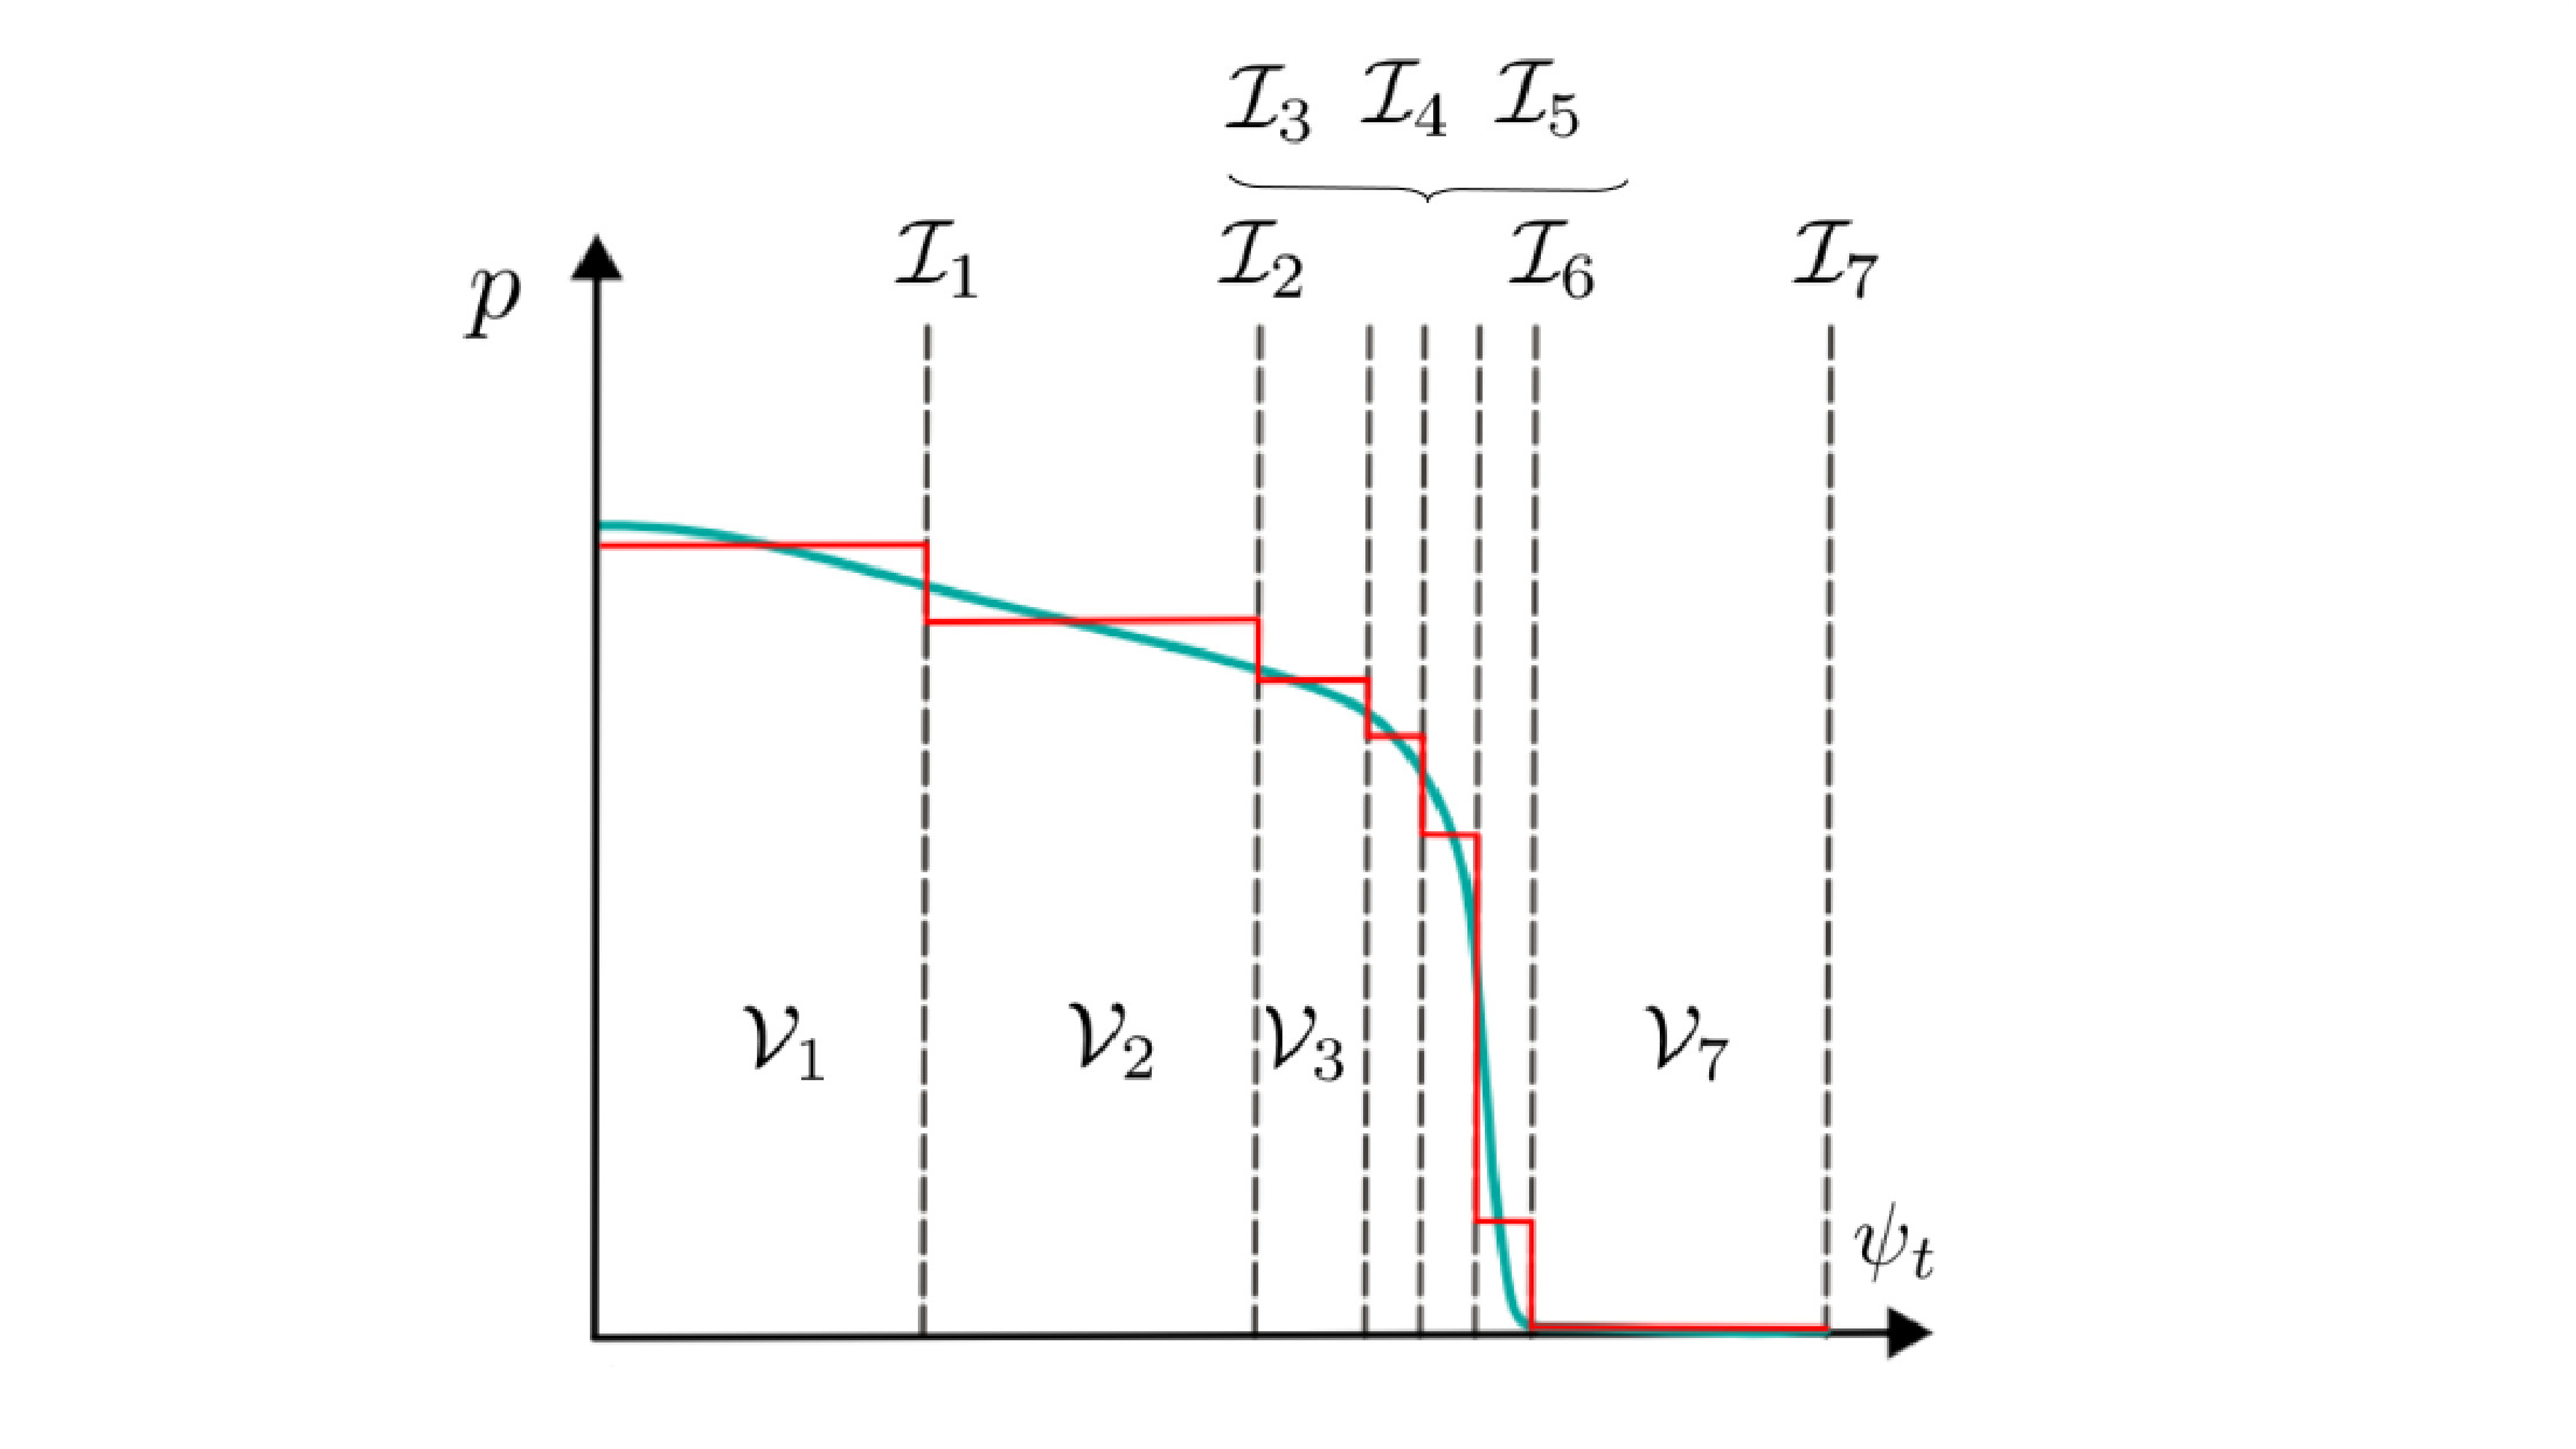
\includegraphics[width=\linewidth]{main/Figures_CurrentConstraint/ABaillod_fig2.pdf}
    \caption{Sketch of a pressure profile as a function of the toroidal flux. Blue: continuous pressure profile obtained via experiment or analytical model. Red: SPEC discretized pressure profile. Black dashed lines: volume interfaces.}
    \label{fig:sketch_pressure}
\end{figure}

A proposed representation of these current density profiles in \ac{MRxMHD} is achieved as follows. The \ac{ECCD} current is an externally driven, parallel current and is thus represented as a volume current since it flows parallel to the field lines; on the other hand, the bootstrap current is a pressure-driven, self-generated current and is represented as a surface current, since it is localized at the pressure gradients. Volume currents are obtained by integrating the externally driven current density in each volume (Figure \ref{fig:sketch_eccd}), which is simply given by the difference

\begin{figure}
    \centering
    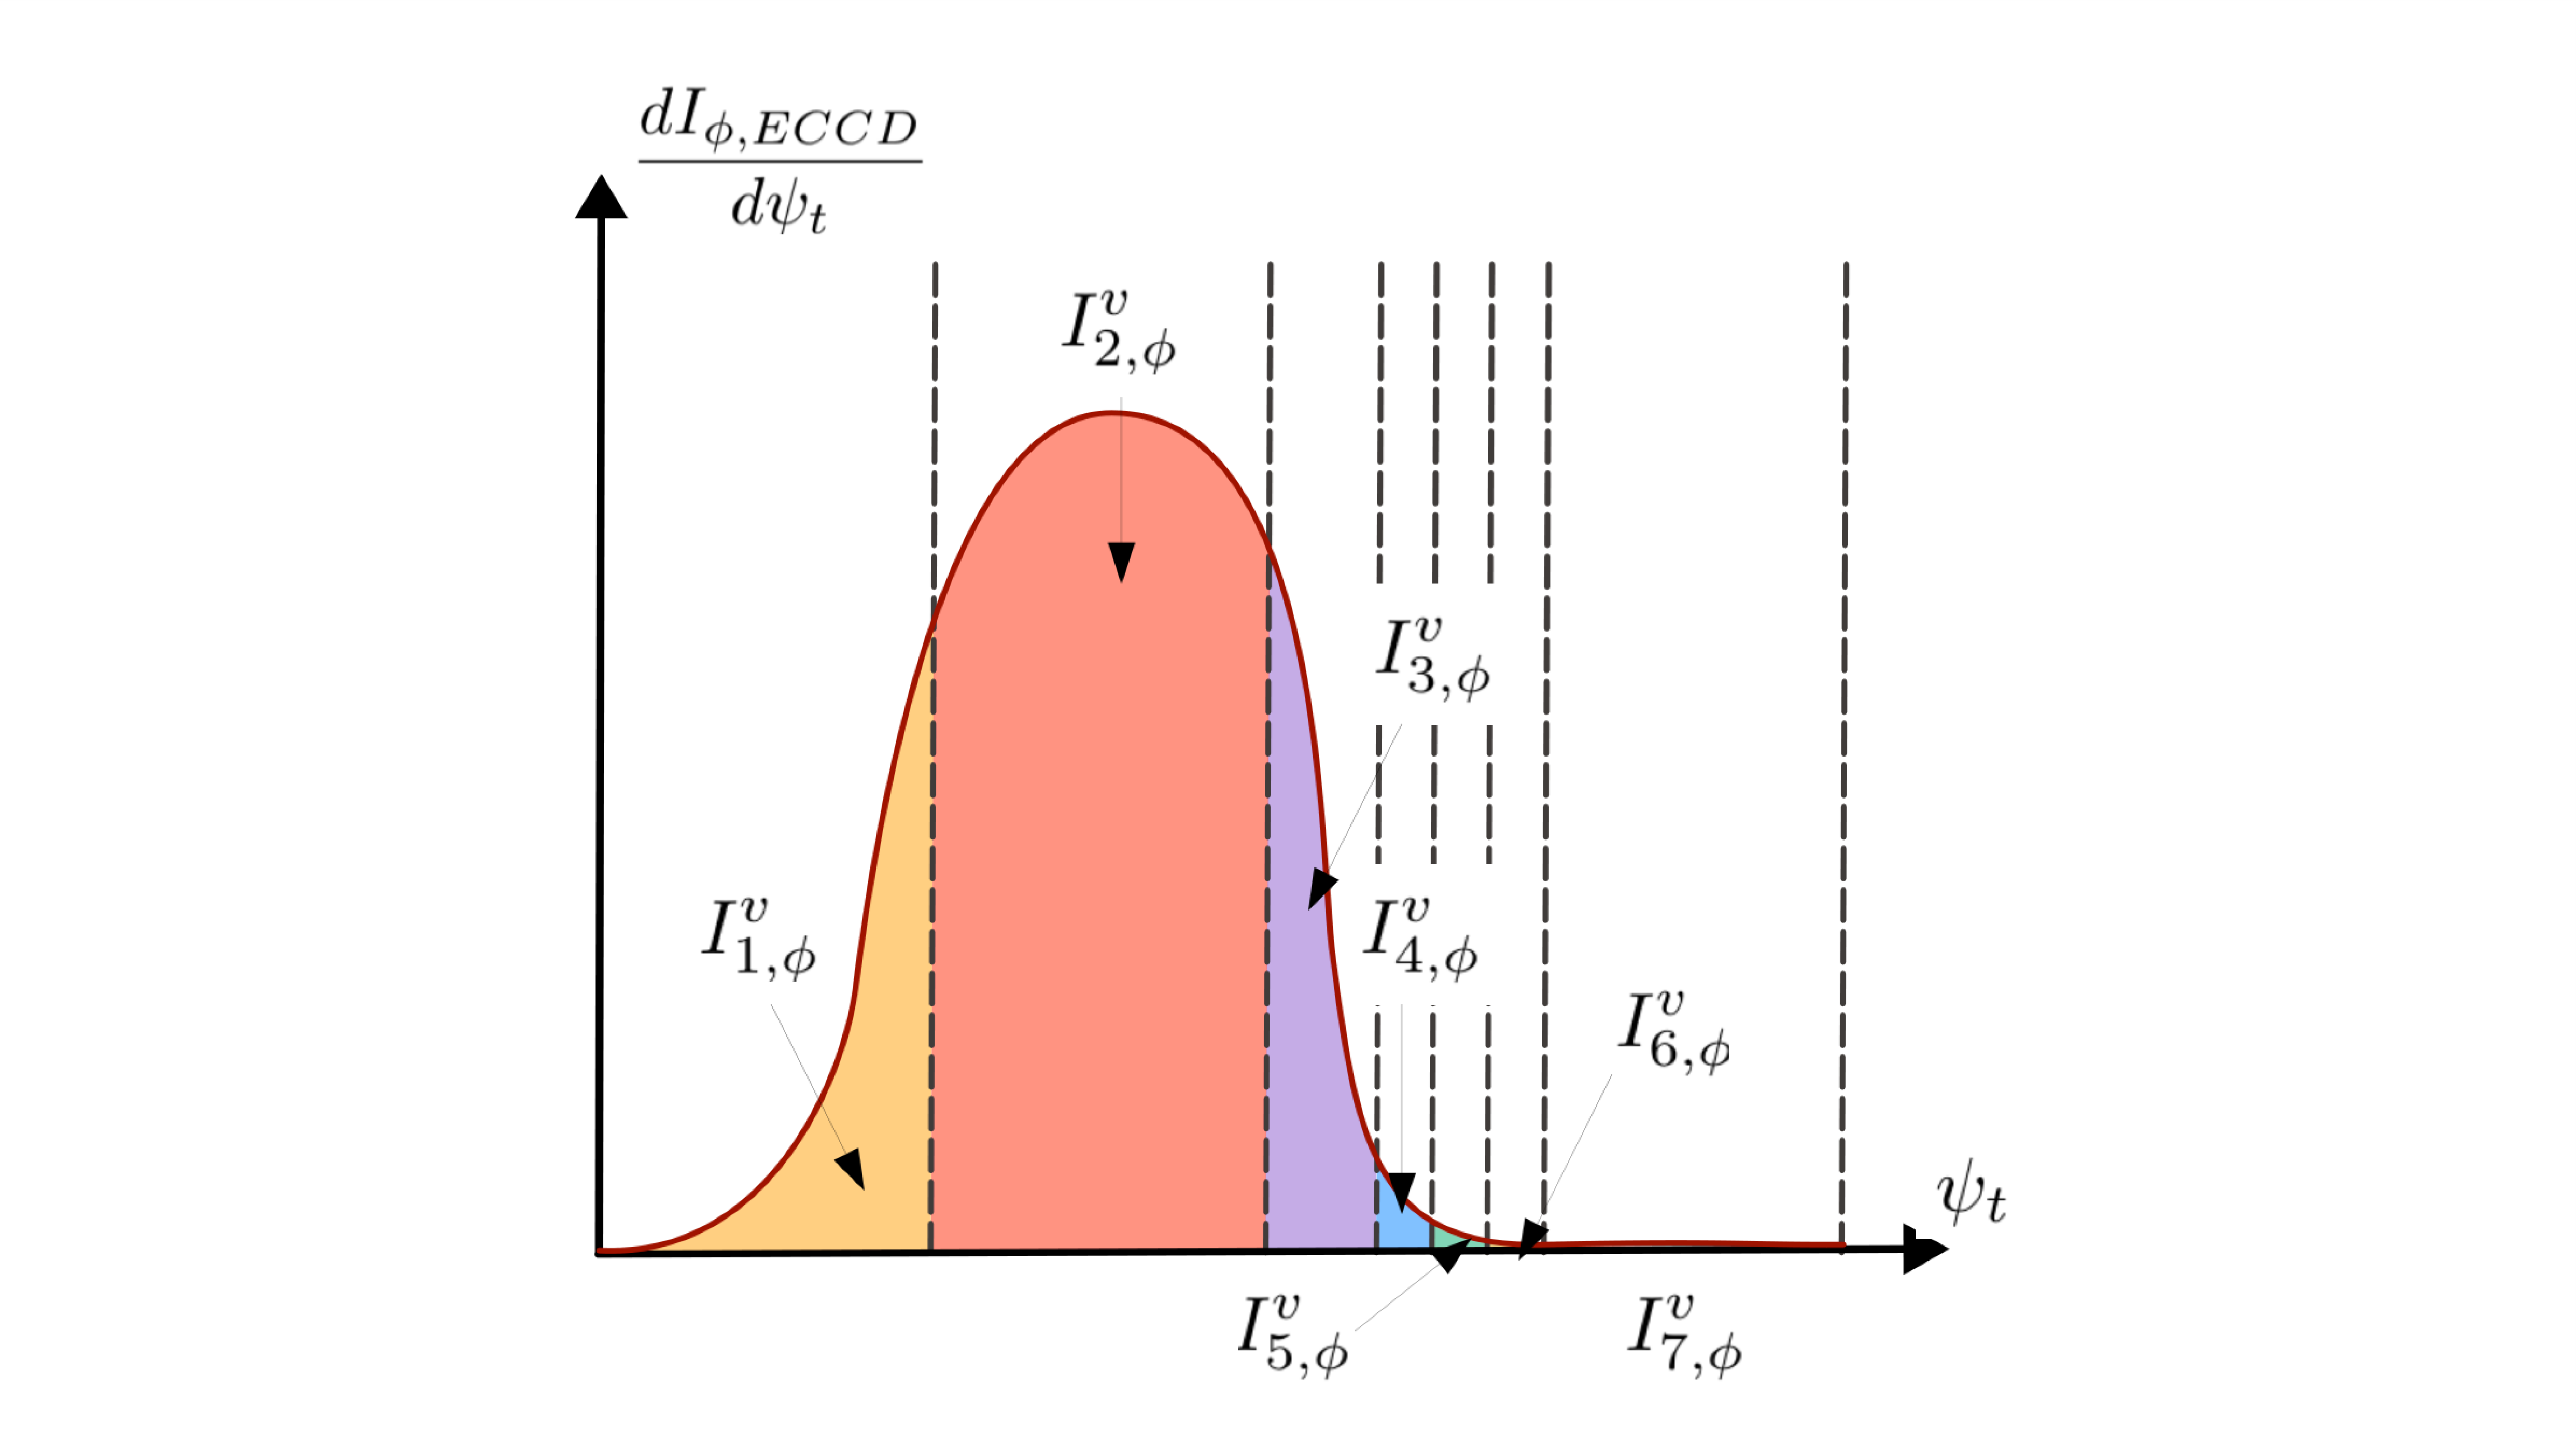
\includegraphics[width=\linewidth]{main/Figures_CurrentConstraint/ABaillod_fig3.pdf}
    \caption{Sketch of externally driven current density (red curve). Colored area correspond to the \ac{MRxMHD} volume current. Black dashed lines represent volume interfaces.}
    \label{fig:sketch_eccd}
\end{figure}


\begin{equation}
    I^v_{l,\phi} = I_{\phi,ECCD}(\psi_{t,l}) - I_{\phi,ECCD}(\psi_{t,l-1}), \label{eq.rep_volume_current}
\end{equation}
and the surface currents are obtained by integrating the pressure driven current density around each interface (Figure \ref{fig:sketch_bootstrap}), which is expressed as

\begin{equation}
    I^s_{l,\phi} = I_{\phi,BS}(\psi_{l,out}) - I_{\phi,BS}(\psi_{l,in}), \label{eq.rep_surface_current}
\end{equation}
with

\begin{align}
    \psi_{l,in} &= \begin{cases}
    0 & \text{if } l=1\\
    \frac{\psi_{t,l-1} + \psi_{t,l}}{2} & \text{otherwise}
    \end{cases}\label{eq.surf_disc1} \\
    \psi_{l,out} &= \begin{cases}
    \psi_{a} & \text{if } l=N_{vol}-1\\
    \frac{\psi_{t,l} + \psi_{t,l+1}}{2} & \text{otherwise}
    \end{cases},\label{eq.surf_disc2}
\end{align}
with $\psi_{a}$ the total toroidal magnetic flux enclosed by the plasma. In Eqs.(\ref{eq.surf_disc1})-(\ref{eq.surf_disc2}), care has been taken for the first and last interfaces, where the surface of integration has been extended to include the current density from the magnetic axis and up to the plasma boundary. Note that this difference in the definition of the first and last surface currents vanishes as the number of volumes $N_{vol}$ is increased. Eqs.(\ref{eq.rep_volume_current})-(\ref{eq.surf_disc2}) are only one possible discretization of the continuous current profiles, proposed by the authors for illustration. Advantages of this particular representation are (1) that the total toroidal current is always preserved and (2) that the currents are approximately localized at the same location in the discretized than in the continuous case. The following sections do not depend on the particular choice of discretization of the currents.


\begin{figure}
    \centering
    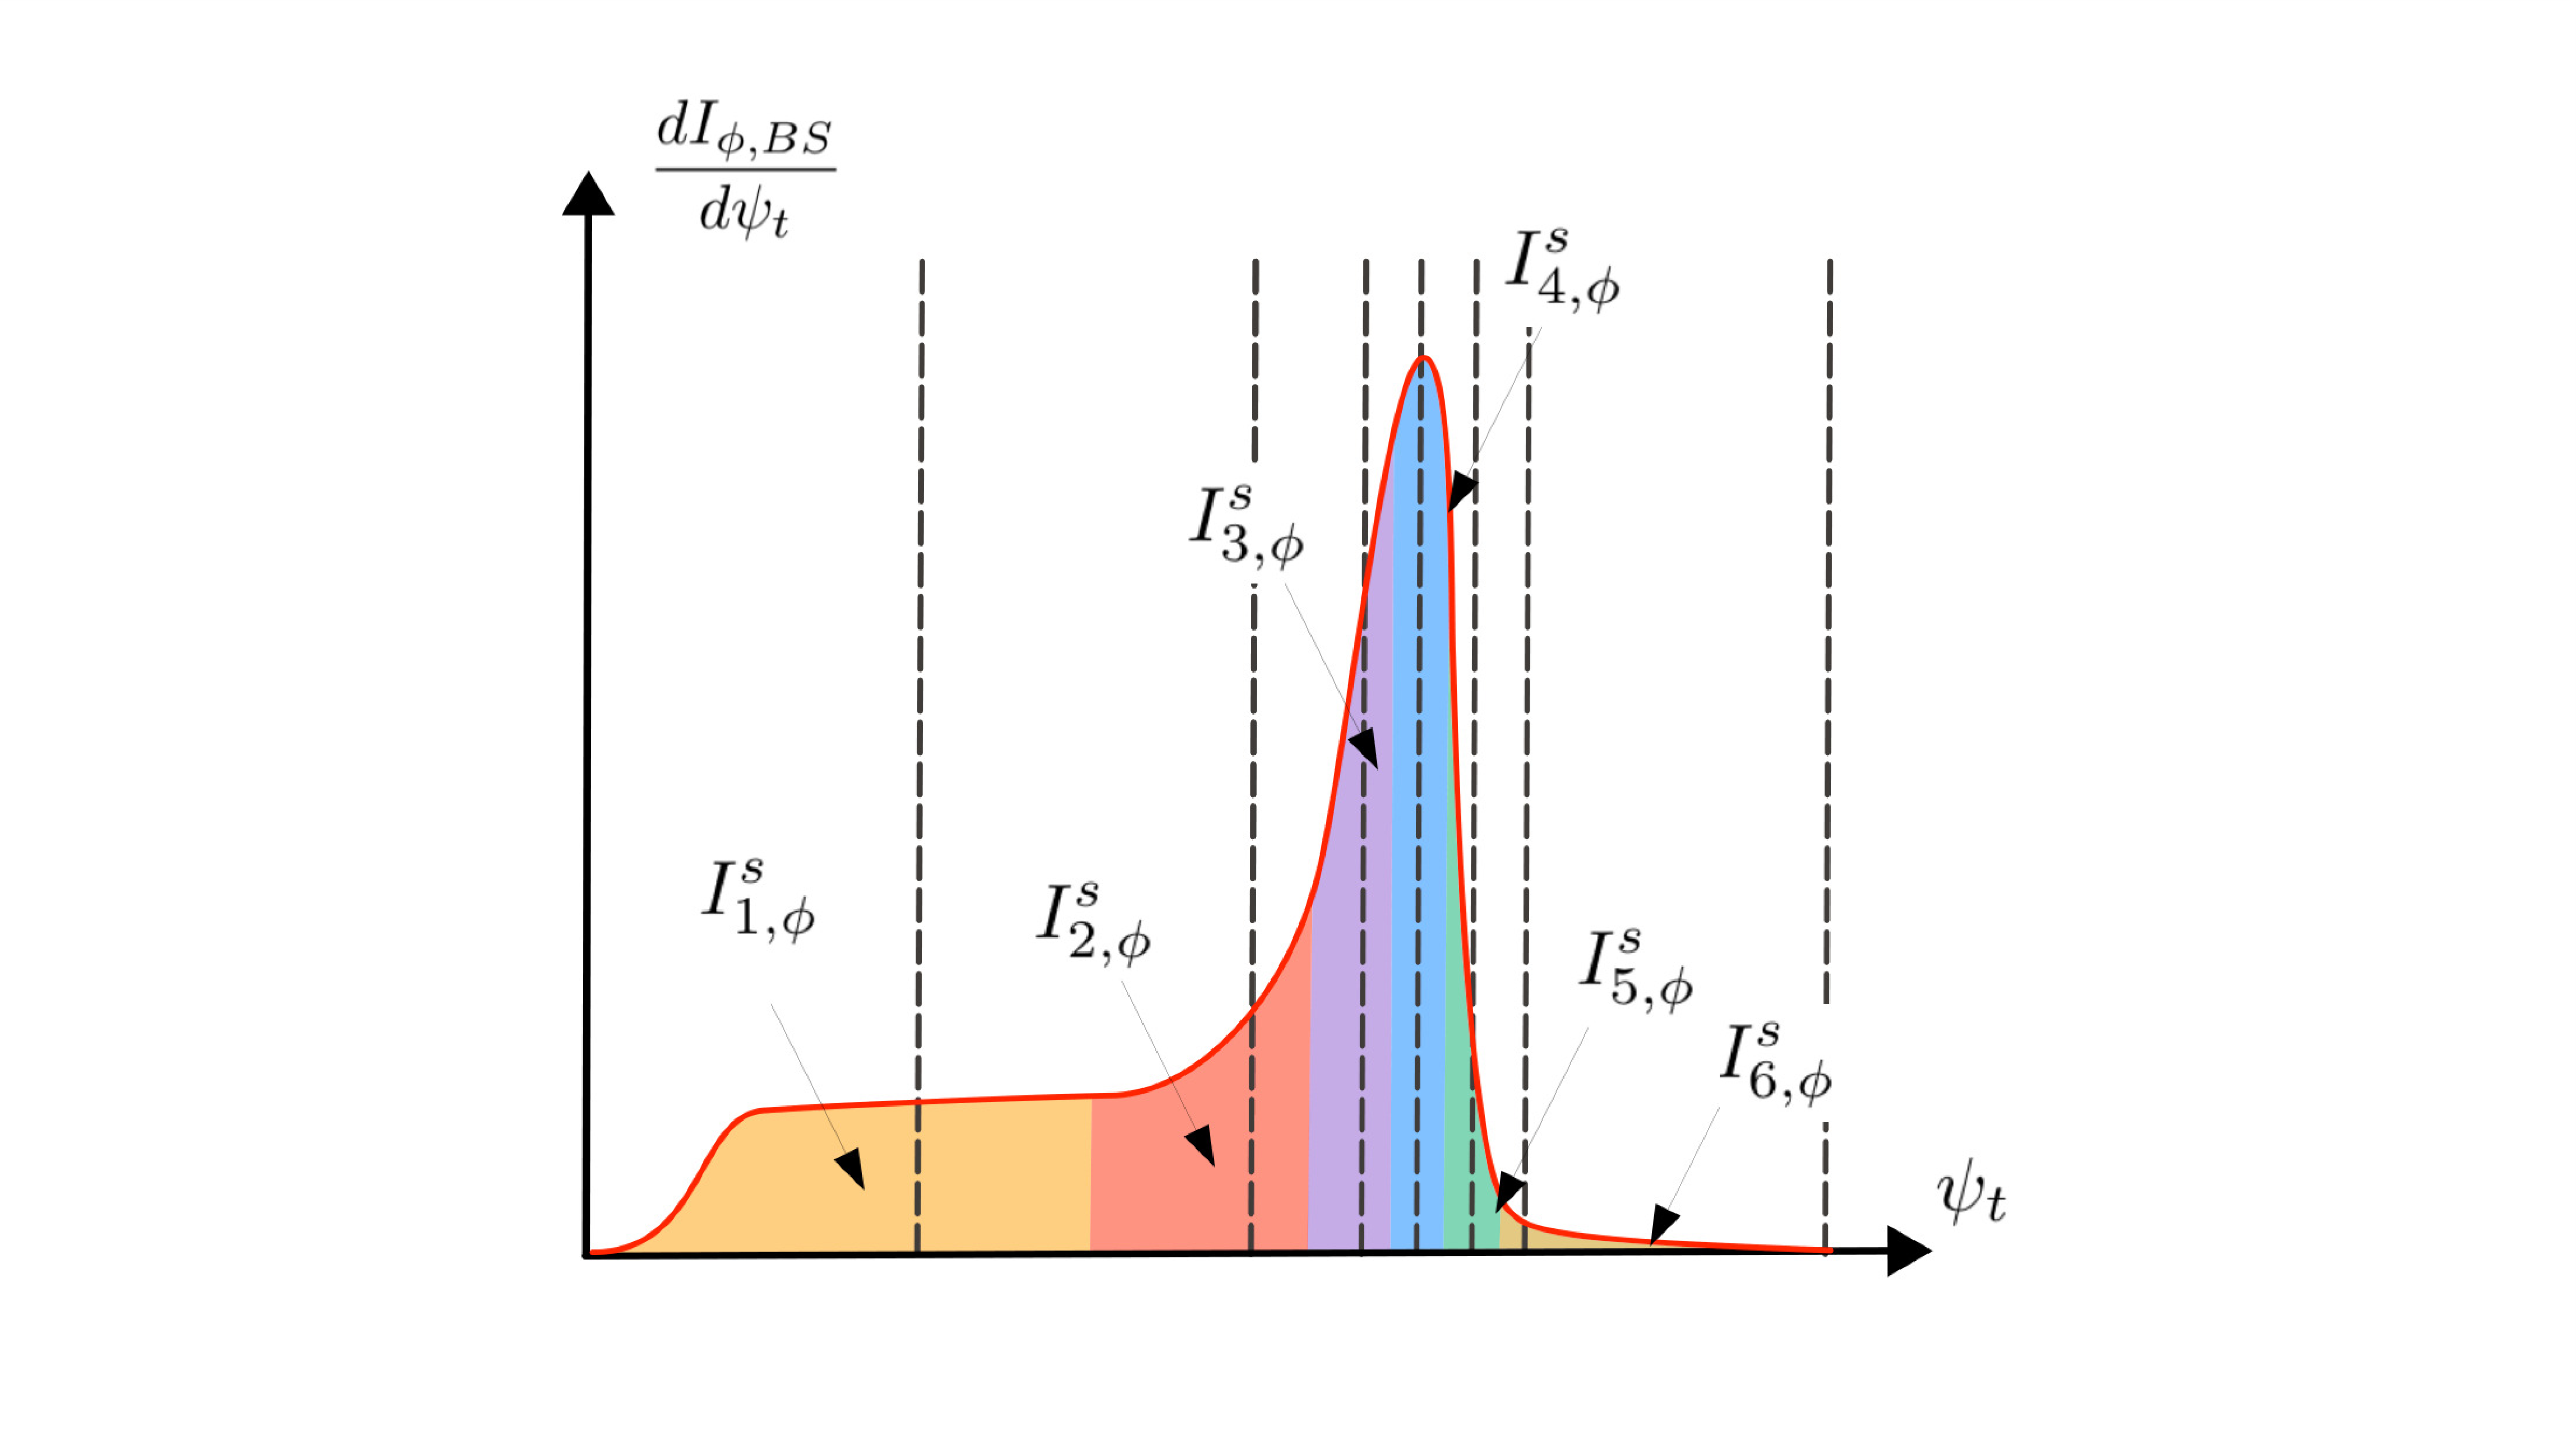
\includegraphics[width=\linewidth]{main/Figures_CurrentConstraint/ABaillod_fig4.pdf}
    \caption{Sketch of pressure driven current density. Colored area correspond to the \ac{MRxMHD} surface current. Black dashed lines represent volume interfaces.}
    \label{fig:sketch_bootstrap}
\end{figure}







\section{Energy principles}
To complete this chapter, we show here that the ideal MHD equilibrium equations, the Taylor state, and the MRxMHD equations can all be derived from an energy principle. In fact, all three models derive from the same energy functional, which is minimized under different topological constraints. We first start by discussing the relation between magnetic helicity and field line topology conservation.

% ================================================ HELICITY ================================================
\subsection{Conservation of field line topology}
%In ideal \ac{MHD}, it is assumed that the plasma is \emph{ideal}, meaning that it has zero resistivity. There are thus no mechanisms for energy dissipation and the plasma is not allowed to reconnect, \textit{i.e.} only plasma displacements that conserve the topology of magnetic field lines are allowed. It has been shown \citep{woltjer_theorem_1958} that this constraint is equivalent to conserving the magnetic helicity $K$ in any plasma volume $\mathcal{V}_i$, with
An important property of the ideal MHD model is that the magnetic helicity $K$ is conserved everywhere under ideal MHD evolution, with
\begin{equation}
	K = \iiint_{\mathcal{V}_i} d\mathbf{x}^3 \mathbf{A} \cdot \mathbf{B},
\end{equation}
where $\mathbf{A}=\nabla\times\mathbf{B}$ is the magnetic vector potential. Indeed, we find
\begin{align}
	\frac{dK}{dt} &= \iiint_{\mathcal{V}_i} d\mathbf{x}^3 \frac{d\mathbf{A}}{dt}\cdot\mathbf{B} + \mathbf{A}\cdot\frac{d\mathbf{B}}{dt} + \iint_{\delta\mathcal{V}_i} \mathbf{A}\cdot\mathbf{B}(\mathbf{n}\cdot\mathbf{v})d\mathbf{x}^2, \\
	&= -2\iiint_{\mathcal{V}_i}\mathbf{E}\cdot\mathbf{B} d\mathbf{x}^3 + \iint_{\delta\mathcal{V}_i}(\mathbf{n}\times\mathbf{A})\cdot(\mathbf{E}+\mathbf{v}\times\mathbf{B})d\mathbf{x}^2.
\end{align}
Applying the ideal Ohm's law (Eq.(\ref{ideal Ohms law})), we obtain $dK/dt = 0$, \textit{i.e.} the magnetic helicity is conserved everywhere in the plasma in ideal MHD. Indeed, the magnetic helicity has been shown to be approximately conserved during fast reconnection events \citep{bergerIntroductionMagneticHelicity1999}, and has been observed to be conserved in tokamak sawtooth crashes \citep{Heidbrink2000}. 

An important property of magnetic helicity is its correlation with magnetic field line topologies. One can show \citep{moffattDegreeKnottednessTangled1969, arnoldTopologicalPropertiesMagnetic1998, bergerIntroductionMagneticHelicity1999} that the magnetic helicity is the sum of the Gauss linking number over every pair of field lines within a volume. Note the following implication: in ideal MHD, the magnetic helicity is conserved \emph{everywhere}, meaning that the magnetic topology is conserved during plasma motion.





% ================================================ ENERGY PRINCIPLE ================================================
\subsection{Energy principle}
The ideal MHD equilibrium equations, Eqs.(\ref{equation perp force balance})-(\ref{equation div B ideal mhd}), can be derived from an energy principle \citep{kruskalEquilibriumMagneticallyConfined1958}. Consider the energy functional 
\begin{equation}
	W = \iiint_{\mathcal{V}_P} d\mathbf{x}^3 \left(\frac{\mathbf{B}^2}{2} + \frac{p}{\gamma-1}\right), \label{eq. energy functional}
\end{equation}
where $\mathcal{V}_P$ is the plasma volume, $d\mathbf{x}^3$ is a volume element, $\mathbf{B}$ is the magnetic field, and $\gamma$ is the ratio of the fluid specific heats. Minimizing $W$ under the constraint of conservation of magnetic helicity everywhere in the plasma leads to the ideal MHD equilibrium equations. 





The plasma is divided in $N_{vol}$ nested volumes $\mathcal{V}_l$, , so that the MHD energy $W_l$ \citep{kruskal_equilibrium_1958} local to each volume can be written as

\begin{equation}
	W_l = \int_{\mathcal{V}_l} \left(\frac{p_l}{\gamma-1}+\frac{B^2}{2\mu_0}\right)dv,
\end{equation}
where $p_l$ is the pressure, $B=|\mathbf{B}|$ is the magnetic field strength, $\mu_0$ is the vacuum permeability, $\gamma$ is the adiabatic constant and $dv$ is an infinitesimal volume element. The \ac{MRxMHD} energy functional is \citep{Hudson2012}

\begin{equation}
	W = \sum_{l=1}^{N_{vol}} \left[W_l -\frac{\mu_l}{2}(K_l-K_{l,0})\right], \label{eq.energy}
\end{equation}
where $\mu_l$ is a Lagrange multiplier, $K_l$ is the magnetic helicity in volume $l$ and $K_{l,0}$ the magnetic helicity constraint. The magnetic helicity is defined as 

\begin{equation}
	K_l = \int_{\mathcal{V}_l} \mathbf{A}_l\cdot \mathbf{B}_l dv,
\end{equation}
where $\mathbf{A}_l$ is the vector potential of the magnetic field  $\mathbf{B}_l$, \textit{i.e.} $\mathbf{B}_l=\nabla\times\mathbf{A}_l$. In each volume $\mathcal{V}_l$, $l\in\{1,\ldots,N_{vol}\}$, the magnetic field $\mathbf{B}_l$ is varied while keeping the toroidal magnetic flux, $\psi_{t,l}$, and poloidal magnetic flux, $\psi_{p,l}$, constant, until the \ac{MRxMHD} energy (Eq.\ref{eq.energy}) is minimized. The corresponding Euler-Lagrange equations \citep{Hudson2012} describe a force-free magnetic field $\mathbf{B}_l$ satisfying a Beltrami equation,

\begin{equation}
	\nabla\times\mathbf{B}_l = \mu_l\mathbf{B}_l.
\end{equation}


\end{document}